\chapter{Power Plant Cost Model Preparation}\label{ch4:cm_prep}

\section{EGS Expansion Concept}\label{ch4:cm_concept}
\subsection{Lightning Dock EGS}

Lightning Dock (Section \ref{ch2:lightning_dock}) is presently the only commercial power plant operating in the state of New Mexico. The net generating capacity after its first phase of development was 4 MW in 2013, with the expectation of upgrading to 10 MW in a second development phase that never came to fruition. Instead, the facility underwent a significant refit in 2018, resulting in a net capacity of 11.2 MW generated entirely from hydrothermal brine production \citep{bonafin_repowering_2019}. 

Department of Energy-funded efforts to characterize the geothermal resources in the Animas Valley, NM revealed the presence of two different thermal reservoirs: the hydrothermal resource targeted by Lightning Dock where deep geothermal fluids ascend along the Animas Valley Fault complex to $\approx$365-1000 m depth, and a secondary interval at $\approx$900-1200 m depth that requires permeability enhancement for production \citep{schochet_development_2001}. The Horquilla limestone formation defines the second reservoir, estimated to span a minimum volume of 6 cubic km based on conservative figures. By one proprietary study completed in 2001 for Ormat Technologies, a commercial geothermal company, the Horquilla has a 88\% probability of 6 MW in recoverable electricity generation potential \citep{schochet_development_2001}.

\citet{schochet_development_2001} proposed the construction of a 6 MW hybrid power plant combining hydrothermal and EGS-sourced power generation a decade before operations commenced at Lightning Dock. In their development plan, they noted several benefits of pursuing EGS in this location:
\begin{itemize}[itemsep=2pt]\label{ch4:ld_egs_support}
    \item Relatively shallow resource drives lower drilling costs
    \item EGS water requirements are attainable from paired hydrothermal operations
    \item A comprehensive initial assessment determined no significant environmental degradation is expected from geothermal operations
    \item Lightning Dock has direct access to in-place transmission lines  
    \item Opportunities exist for electricity sales to local users
    \item Purchase agreements with regional utilities are incentivized by NM legislation
\end{itemize}

As suggested by this list, the conditions at Lightning Dock offer a nearly ideal test case for an EGS proof of concept on a manageable scale. Historical land utilization in the area is primarily agricultural with few residences, so risk is low for any adverse impact on an existing population. In addition, use of a binary cycle design as proposed by \citet{schochet_development_2001} offers the potential for power production with zero GHG emissions.  

In this thesis, the \citeauthor{schochet_development_2001} concept is revisited with the existing geothermal production at Lightning Dock kept in mind; rather than building a new hybrid facility, the revised concept involves targeting the deeper reservoir as a near-hydrothermal field EGS (NF-EGS) development with a tie-back to the current Lightning Dock facility. Stepping out from the hydrothermal zone in proximity to the Animas Valley Fault complex, thermal conditions settle to a high background geothermal gradient between $\approx$ 80-120 K/km based on boreholes TG 56-14 and TG 12-7 \citep{cunniff_final_2003} -- certainly high enough to support geothermal capture. These conditions make for an interesting case study on risk mitigation options for EGS production planning.

Public records regarding power generation at Lightning Dock provide some guidance on the appropriate size for an EGS expansion. After phase 1 development, the plant produced 4 MW. An additional 6 MW was slated for phase 2, but re-powering of the plant actually added 7 MW to the capacity after several years of development stasis \citep{think_geoenergy_turboden_2020}. \citeauthor{schochet_development_2001} originally proposed a 6 MW hybrid plant for the site, but they also noted 6 MW from the Horquilla was likely understating the full reservoir potential \citeyear{schochet_development_2001}. In consideration of the step-wise trajectory of plant improvements and assessment of available thermal resource, this case study targets 5 MW as a expansion goal. 

\subsection{New Mexico Electricity Demand}

Pursuing the expansion of a power plant requires sufficient demand to ensure total revenue offsets project expenses. Fortunately, New Mexico regulations support the further development of geothermal power production in the state. Specifically, the Energy Transition Act signed in 2019 updated the New Mexico \acrlong{rps} (\acrshort{rps}) to go zero-carbon by 2050, with milestone targets along the way \citep{lillian_new_2019}. The RPS dates back to the Renewable Energy Act passed in 2004 and comes with several carve-outs, including a 30\% requirement for wind energy, 20\% for solar, and 5\% for other renewables like geothermal \citep{dsire_dsire_2021}. Public Service Company of New Mexico (PNM) is the state’s largest energy provider and services the Lordsburg area where Lightning Dock is located. PNM and Cyrq Energy currently share a 20-year \acrlong{ppa} (\acrshort{ppa}) for electricity generated at Lightning Dock. The PPA has gone through amendments over time to update both the wattage supplied to PNM and the pricing structure per MWh \citep[e.g.,][]{pnm_public_2014,stanfield_new_2017}. This indicates a PPA can be revisited if conditions change, which is an important aspect to consider when modeling project financials. 
In addition to the RPS requirement for a diversified renewables portfolio, coal power plants across the state face mandated shut-downs as a consequence off the Energy Transition Act. Coal currently supplies a large fraction ($\approx$ 45\%) of electric power sector consumption in New Mexico (Figure \ref{fig:nm_energy_consumption}). The supply gap introduced as coal-based production ramps down to zero could more than compensate for a 5 MW addition of no-emissions energy to the New Mexico grid.

\begin{figure}[!htp]
\centering
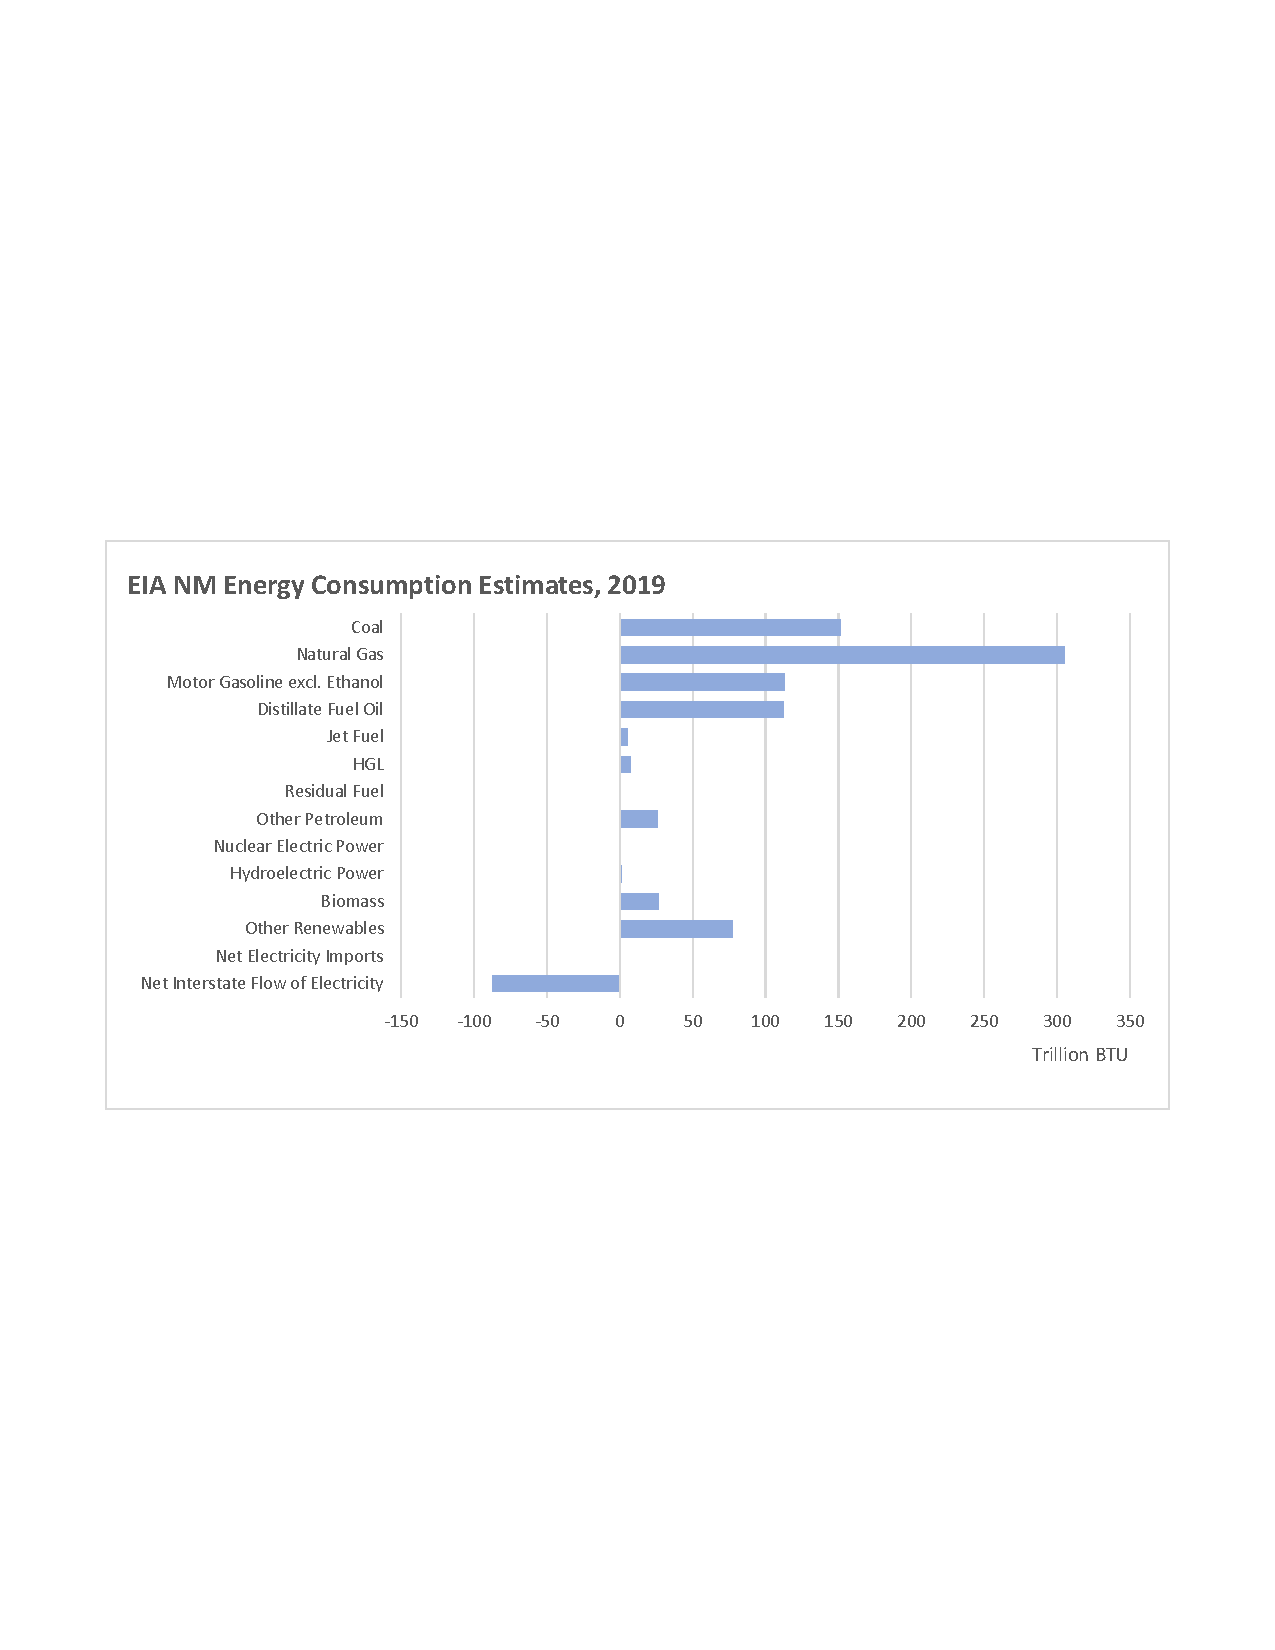
\includegraphics[width=\textwidth]{templates/images/Figure-EIA_NM_Energy_Consumption.pdf}
\caption[NM energy consumption]{Energy consumption by source for New Mexico. Adapted from data and graphics reported by the EIA \protect\citep{eia_new_2021}.}
\label{fig:nm_energy_consumption}
\end{figure}

\subsection{Modular Geothermal}
Limiting this expansion to a single 5 MW facility represents one design alternative, but others exist as well. One flexible option uses modular technology that recently captured the attention of high-stakes investors across the world \citep{shieber_bill_2019}. Climeon has engineered a compact binary cycle unit capable of 150 kW of generated electricity using inlet fluid temperatures rated up to 120℃ and flow rates of up to 35 kg/s \citep{climeon_climeon_2021-1}. These units can be combined into a larger deployable Power Block for 1050 kW of generated electricity \citep{winther_power_2018} (Figure \ref{fig:climeon_powerblock}). Using this technology, power plants can now be treated like multi-unit assemblages, installed all at once or over an extended period of time based on operator needs \citep{climeon_why_2018}.

\begin{figure}[!htp]
\centering
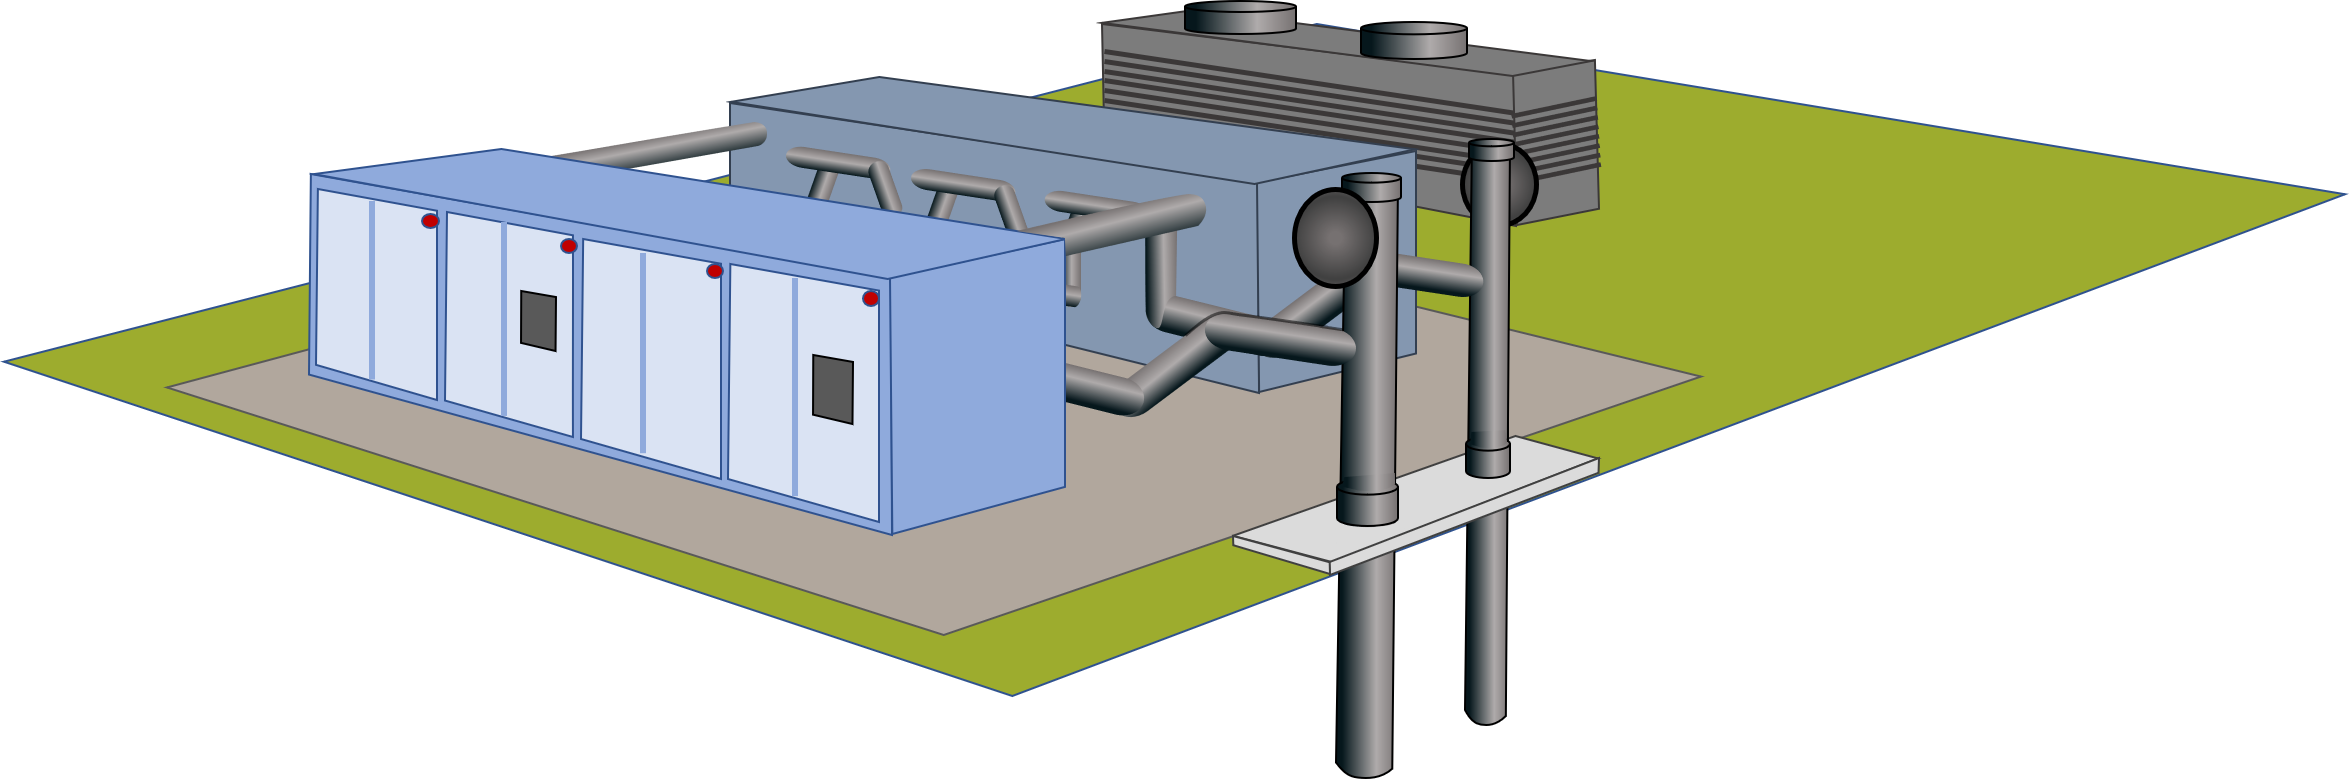
\includegraphics[width=\textwidth]{templates/images/Figure-Climeon-PowerBlock.png}
\caption[Modular power plant schematic]{Modular binary cycle power plant concept, adapted from Climeon PowerBlock schematic diagram \protect\citep{climeon_climeon_2021-1}. Each block consists of seven active units chained together for $\approx$1 MW of generating capacity.}
\label{fig:climeon_powerblock}
\end{figure}

\subsection{Flexibility with Real Options}
As discussed in Section \ref{ch2:costmod}, cost models can provide insights into the potential value gained or lost by a proposed facility before construction even begins. Well-established geothermal cost models like GETEM \citep{entingh_volume_2006} present a highly parameterized but deterministic view of cost and investment opportunity given a defined geothermal resource and development concept. Other models may apply different assumptions or mathematical treatments for various facets of the system, however they uniformly offer a single-track aspect to how the project unfolds over its lifecycle. Users can test ideas, but the solution space remains under-explored due to implicit assumptions of variable trends or static behaviors for a highly-dynamic system.  

In the cost model outlined below, the economic analysis incorporates uncertainty by replacing single value estimates with distributions for model variables. This enables the model to produce a representative range of possible outcomes when simulated many times over. In addition, the model flexibly adapts by executing real (engineering) options, where design updates triggered by changing conditions allow the system to realize upside potential or characterize the extent of downside risk. Designs need not be static, and real options can greatly increase the expected value of a project by exploring execution strategies otherwise missed by more traditional modeling approaches \citep[chap.6]{de_neufville_flexibility_2011}.

\section{Cost Model Structure}
\label{ch4:cm_structure}

Geothermal cost models typically report Levelized Cost of Electricity (LCOE) for simple comparison with other renewable energy sources. However, LCOE is standardized to represent the total lifetime costs incurred by a power plant normalized by the total power generation from start-up to plant decommissioning. LCOE is thus not well-suited for communicating projected gains or losses under different plant designs or scenarios, which are the focus of this analysis. Instead, the model described here relies on \acrlong{npv} (\acrshort{npv}), a simple measure of project lifetime worth that accounts for the time value of money by applying a single interest rate, the discount rate, for both borrowing and deposits \citep[p.\ 195-215]{de_neufville_flexibility_2011}. Here, "present value" refers to a 2020 cost basis. For power generation over a 30-year lifespan -- the default for geothermal models like GETEM \citep{entingh_volume_2006} -- this basis takes the model out to 2050, a common benchmark year for future projections. 

\subsection{NPV Model}
\label{ch4:cm_npv}
Following the general outline for geothermal cost modeling from previous work \citep[e.g.,][]{augustine_hydrothermal_2009, beckers_introducing_2013,tester_future_2006}, this thesis considers revenue (R), operating \& maintenance costs (OpEx or OM), and capital expenditures (CapEx or C) as the primary components defining annual cash flow (see Equation \ref{eq:cm_components}). Capital expenses can be further decomposed into five  sub-components associated with exploration, drilling \& completions, reservoir stimulation, fluid distribution, and power plant costs. Likewise, operating expenses subdivide into subsidiary costs for the power plant, wells, and water management.

\begin{equation}
    \label{eq:cm_components}
    \begin{aligned}
    NPV &= \sum_{t=1}^{T}D_t \cdot \left( R_t - C_t - OM_t \right)\\
    \text{where:}\\
    C_t &= \left[C_{expl} + C_{dc} + C_{stim} + C_{dist} + C_{pp}\right]_t\\
    OM_t &= \left[OM_{pp} + OM_{well} + OM_{water}\right]_t
    \end{aligned}
\end{equation}
\\
Revenue and expenses are treated on an annual basis, meaning shorter-term fluctuations like price and production seasonality are not explicitly modeled. $D_t$ in Equation \ref{eq:cm_components} defines the time-based conversion factor between cash flow for a specific year and discounted cash flow for the basis year (see Equation \ref{eq:discount_rate}).

\subsubsection{Revenue} \label{ch4:cm_rev}

Calculations of undiscounted revenue require an estimate of the electricity produced within a year ($W$) and the price set by a power purchase agreement ($p_{PPA}$) for that electricity \citep{entingh_volume_2006}. 

\begin{equation}
    \label{eq:cm_rev}
    R = W \cdot p_{PPA} = (b_e \cdot \dot{m}) \cdot p_{PPA}
\end{equation}
\\
Brine effectiveness ($b_e$) describes the electricity output per unit flow of produced brine ($\dot{m}$) and depends on the production temperature of the brine. The GETEM model uses an empirical correlation between the brine temperature ($^\circ$C) and effectiveness (w-hr/kg) \citep[p.\ 62]{entingh_volume_2006}:

\begin{equation}
\begin{aligned}
    \label{eq:brine_eff}
    b_e &= C_0 + C_1 \cdot T_{prod} + C_2 \cdot T_{prod}^2 + C_3 \cdot T_{prod}^3 + C_4 \cdot T_{prod}^4 \\
    &\quad C_0 = 9.41376 \\
    &\quad C_1 = -0.182542 \\
    &\quad C_2 = 0.0001765735 \\
    &\quad C_3 = 0.000012204486 \\
    &\quad C_4 = -0.0000000335559
\end{aligned}
\end{equation}

In the GETEM interface, a user selects to determine the electricity output for a specified input temperature and flow rate, or alternatively, derive the required flow rate to meet a pre-determined power sales capacity at the same input fluid temperature \citep{entingh_volume_2006}. Since the Climeon analog has a known net capacity of 150 kW per unit or 1.05 MW for each PowerBlock, and standard flow rates are provided in models like GETEM, both options are explored in this thesis.

\subsubsection{Exploration Capital Expenses} 
\label{ch4:cm_capex_expl}
Costs for exploration activities are estimated by the same method defined for the 2012 GETEM model (Equation \ref{eq:cm_capex_expl}) \citep{eere_getem_2012}. 

\begin{equation}
\label{eq:cm_capex_expl}
    C_{expl} = PPI \cdot \left[ 1.12 \cdot (\$1\text{M} + 0.6\cdot C_{dc}) \right]
\end{equation}

This relationship assumes slim hole (3-6" diameter) drilling for exploration at a 60\% discounted cost compared to standard-sized ($\geq$ 8.5" diameter) geothermal wells. The constant \$1M term accounts for pre-drilling costs, including field work, geophysical surveys of field structure, and interpretation of results. Technical and office support is covered by an additional 12\% applied to the estimate \citep{eere_getem_2012}. Total exploration costs are converted to a 2020 cost basis using the Producer Price Index (PPI) for electric power generation from the U.S. Bureau of Labor and Statistics \citep{us_bls_ppi_2021}.

\subsubsection{Drilling \& Completions Capital Expenses} 
\label{ch4:cm_capex_dc}

Geothermal drilling and completions costs differ from traditional oil \& gas wells due to differences in hole diameter, thermal and geochemical conditions, and the strength and abrasiveness of the target formations \citep{lowry_geovision_2017}. Here, drilling capital expenditures rely on a cost curve described by \citet[Equation 4,\ ][]{beckers_introducing_2013}.

\begin{equation}
\label{eq:cm_cdc}
    C_{dc} = PPI \cdot \left[ 1.65 \cdot 10^{-5} \cdot \text{MD}^{1.607} \right]
\end{equation}
\\
where $C_{dc}$ is measured in \$M and MD refers to well measured depth in meters. Each power plant module will require an injector-producer pair, so this represents one-half of the drilling cost per module. Drilling costs are converted to a 2020 cost basis using the industry index for electric power generation \citep{us_bls_ppi_2021}. 

Note that Equation \ref{eq:cm_cdc} was derived for well depths of 1600-9000 m. Assuming an average geothermal gradient of 100 K/km (Table \ref{tab:cm_resource_params}), the wells considered for this study could extend slightly shallower than this range, so this should be viewed as a minimum drilling \& completions estimate. The stochastic model considered later in this study includes variability in both geothermal gradient and drilling costs for a more comprehensive treatment of both variables.

\subsubsection{Simulation Capital Expenses}
\label{ch4:cm_stim}

EGS at Lightning Dock requires stimulation of the Horquilla reservoir to create fluid pathways for thermal extraction. The stimulation cost estimate used in this study comes from the recent GeoVision analysis \citep{lowry_geovision_2017}:

\begin{equation}
\label{eq:cm_capex_stim}
    C_{stim} = \$1,250,000
\end{equation}

Since this represents a recent ballpark estimate, no cost basis conversion was applied in the model. In fact, the value in Equation \ref{eq:cm_capex_stim} may be high since it includes the cost of water, which may not be a factor at Lightning Dock with the availability of hydrothermal brine from adjacent power plant operations. The model assumes stimulation is only performed for the injection well in each injector-producer pair, so this represents a \textit{per module} value.

\subsubsection{Distribution Capital Expenses}
\label{ch4:cm_capex_dist}

Fluid distribution costs include the entire surface piping system between the wells and power plant modules. This study uses the same estimate included in the GEOPHIRES model \citep{beckers_introducing_2013}.

\begin{equation}
\label{eq:cm_dist}
    C_{dist} = PPI \cdot \left[ \$50,000 \cdot q_{in} \right]
\end{equation}
\\
where $q_{in}$ is the heat input from the produced brine and $PPI$ converts this 2012 value to a 2020 cost basis. 

The 2nd law or thermodynamic efficiency ($\eta$) governs how much heat from the input fluid can be converted to work. \citeauthor{beckers_low-temperature_2016} provides an estimate for subcritical ORC power plants as follows \citeyear[p.\ 39-41]{beckers_low-temperature_2016}:

\begin{equation}
\begin{aligned}
    \label{eq:2ndlaw_eff}
    \eta &= K_1 \cdot T_{prod} + K_0 \\
         &= 0.002713 \cdot T_{prod} - 0.0918
\end{aligned}
\end{equation}

Combining Equations \ref{eq:cm_dist} and \ref{eq:2ndlaw_eff} allows distribution costs to be calculated in terms of electricity production:

\begin{equation}
\label{eq:cm_dist_eta}
    C_{dist} = PPI \cdot \left[ \$50,000 \cdot W \cdot (0.002713 \cdot T_{prod} - 0.0918) \right]
\end{equation}
\\
where W is the electricity output. Under the scenario where modular power plant units are pre-fabricated and directly provided by a company like Climeon, fluid distribution may be included in the installation fees. Distribution capital expenditures would therefore be subsumed by power plant costs and $C_{dist}$ would reduce to zero. However, without confirmation of the fee break-down structure from Climeon, the model described here relies on Equation \ref{eq:cm_dist_eta}. 

\subsubsection{Power Plant Capital Expenses}
\label{ch4:cm_capex_pp}

Power plant costs for a modular installation remain a source of significant uncertainty for this cost model. The GEOPHIRES model implements a temperature-variable cost estimate first described by \citet{tester_future_2006} for a binary cycle power plant \citep{beckers_introducing_2013}. \citet{schochet_development_2001} predicted produced fluid temperatures of 280-320$^\circ$F (137-160 $^\circ$C) for the Lightning Dock EGS reservoir, which equates to \$1565-\$1694 per kW by the GEOPHIRES estimate. Converted to a 2020 cost basis \citep{us_bls_ppi_2021}, this amounts to \$2230-\$2415 per kW.

If power plant capacity is modularized with pre-fabricated units like the Climeon PowerBlock concept, economies of scale should reduce the cost of construction and installation. Unanswered company inquiries left this rationale unconfirmed. Nevertheless, the author chose to assume a round-number estimate accounting for a modularity discount (Equation \ref{eq:cm_pp}). This could be replaced by more accurate numbers when those values become available.

\begin{equation}
\label{eq:cm_pp}
    C_{pp} = \$2,000 \cdot W
\end{equation}
\\
where W is the electricity output of the plant in kW and $C_pp$ is measured against a 2020 cost basis. Pump costs are assumed to be included in this expense.

\subsubsection{Power Plant Operating Expenses}
\label{ch4:cm_opex_pp}

Power plant operating expenses follow the relationship used by the GEOPHIRES model based on a previous GETEM formulation \citep[Equation 9,\ ][]{beckers_introducing_2013}.

\begin{equation}
\label{eq:cm_om_pp}
    OM_{pp} = 0.75 \cdot C_{labor} + 0.015 \cdot C_{pp}
\end{equation}

Here, $C_{labor}$ refers to labor costs scaled to power plant production. The values in Table \ref{tab:labor_costs} follow \citet[Equation 10,\ ][]{beckers_introducing_2013}, updated to a 2020 cost basis using the Employment Cost Index (ECI) for total compensation for private industry utilities workers \citep{us_bls_eci_2021}.

\begin{table}[!htp]
\centering
\begin{tabular}{|c|c|}
\hline
\textbf{Electricity Output (MW)} & \textbf{Labor Costs (2020 \$)} \\ \hline
\textless 5 & 326,000 \\ \hline
{[}5, 10) & 1,073,000 \\ \hline
{[}10, 20) & 1,460,000 \\ \hline
{[}20, 40) & 2,167,000 \\ \hline
40+ & 2,581,000 \\ \hline
\end{tabular}
\caption[Power plant labor costs]{Power plant labor costs by plant capacity  \protect\citep{beckers_introducing_2013}}
\label{tab:labor_costs}
\end{table}

\subsubsection{Well Operating Expenses}
\label{ch4:cm_opex_well}

Operations and maintenance costs per geothermal well combines labor with a fraction of the drilling \& completions expenses \citep[Equation 12,\ ][]{beckers_introducing_2013}.

\begin{equation}
\label{eq:cm_om_well}
    OM_{well} = 0.25 \cdot C_{labor} + 0.01 \cdot C_{dc}
\end{equation}
\\
where $C_{labor}$ refers to labor costs in Table \ref{tab:labor_costs}. Equation \ref{eq:cm_om_well} covers expenses for a single well and must be doubled for injector-producer pairs associated with each power plant module.

\subsubsection{Water Operating Expenses}
\label{ch4:cm_opex_water}

Water expenses refer to make-up water that replaces subsurface losses to the reservoir. The value applied here comes directly from the GETEM model \citep{eere_getem_2012}.

\begin{equation}
\label{eq:cm_om_water}
    OM_{water} = PI \cdot \left[\$300 \cdot V_{loss}\right]
\end{equation}
\\
where $V_{loss}$ is water loss in units of acre-feet and $PI$ converts this estimate to a 2020 cost basis. This operating cost could be alleviated by directly using excess water from the Lightning Dock hydrothermal operations. The cost model includes it for a more conservative cost estimate, but there is an argument to remove this cost entirely.

\subsection{Rate Calculations}
\label{ch4:rate_calc}

The cost model considers four rates when performing the NPV calculation.

\subsubsection{Discount Rate}
\label{ch4:discount_rate}

Discount rate defines the time value of money and is held constant throughout the 30-year time period being modeled. Equation \ref{eq:discount_rate} describes how discount rate re-scales cash flow to a present "discounted" value for the basis year \citep[p.\ 199]{de_neufville_flexibility_2011}.

\begin{equation}
    \label{eq:discount_rate}
    DCF = \frac{CF}{(1+r)^n}
\end{equation}
\\
where $DCF$ is discounted cash flow, $CF$ is the cash flow for a specific year,  $r$ is the discount rate, and $n$ represents the number of years between the modeled year and the basis year. Combining this relationship with Equation \ref{eq:cm_components}, $(1+r)^{-t}$ replaces $D_t$ as the discount term needed to calculate $NPV$.

\subsubsection{Learning Rate}
\label{ch4:learn_rate}

Learning rate defines the improvement in cost as a result of accumulated knowledge and experience from repeatedly performing an action. In this model, a learning rate only applies to the drilling \& completions costs for EGS wells in the expansion project area. Drilling costs progressively decrease based on the following relationship \citep[p.\ 213]{de_neufville_flexibility_2011}:

\begin{equation}
    \label{eq:learning_rate}
    U_i = U_1 \cdot i^B
\end{equation}
\\
where $U_1$ and $U_i$ are the costs to drill the first and $i^{th}$ wells, respectively, $i$ is the total well count, and $B$ is the slope of the empirically-derived learning rate curve.

\subsubsection{Thermal Drawdown Rate}
\label{ch4:drawdown_rate}

The thermal drawdown rate defines the progressive cooling of the stimulated geothermal reservoir over time. In the model, the reservoir temperature, and hence the temperature of the produced geothermal brine, decreases with each year of continued production by the relationship defined for GETEM (Entingh et al., 2006).

\begin{equation}
    \label{eq:drawdown}
    T_n = T_0 \cdot (1-d)^n
\end{equation}
\\
where $T_0$ and $T_n$ are reservoir temperatures at time 0 and n, $d$ is thermal drawdown rate, $n$ is number of years since drilling and stimulation activities last took place.

\subsubsection{Capacity Factor Degradation Rate}
\label{ch4:degrade_rate}

The NREL Cost of Renewable Energy Spreadsheet Tool (CREST) incorporated an additional capacity factor degradation rate separate from thermal degradation of the resource when modeling geothermal LCOE \citep{gifford_crest_2013}. This rate accounts for natural long-term production degradation of plant performance over the lifetime of the asset. In this cost model, capacity factor degradation is modeled by reducing the capacity factor as the plant ages by applying a relationship similar to Equation \ref{eq:drawdown} for thermal drawdown:

\begin{equation}
    \label{eq:degradation}
    C_n = C_0 \cdot (1-a)^n
\end{equation}
\\
where $C_0$ and $C_n$ are power plant capacity factors at years 0 and n, $a$ is the degradation factor, and $n$ is number of years since the power plant commenced operations.

\subsection{Model Parameters}
In order to estimate the values for the NPV model components, several parameters related to resource recovery, field and plant operations, and key economic factors were chosen for the cost model. The selected parameters are representative of the Lightning Dock area and limits on components of the system to the best of the author's knowledge.

\subsubsection{Resource recovery parameters}

\begin{table}[!htp]
\centering
\resizebox{.9\textwidth}{!}{
\begin{tabular}{|l|c|l|}
\hline
\multicolumn{1}{|c|}{\textbf{Parameter}} & \textbf{Value} & \multicolumn{1}{c|}{\textbf{Source}} \\ \hline
Ambient surface temperature & 15.8 $^\circ$C & \citep{dahal_evaluation_2012} \\ \hline
Average geothermal gradient & 100 K/km & \citep{crowell_history_2014} \\ \hline
Initial average reservoir temperature & 149 $^\circ$C & \citep{schochet_development_2001} \\ \hline
Cooling in production well & 7.5\% & \citep{lowry_geovision_2017} \\ \hline
Flow rate per producer & 40 kg/s & \citep{entingh_volume_2006} \\ \hline
Thermal drawdown rate & 0.5\% & \citep{entingh_volume_2006} \\ \hline
Water loss rate & 2\% & \citep{freeman_system_2018} \\ \hline
\end{tabular}}
\caption[Cost model parameters for resource recovery]{Parameters related to resource recovery in the cost model}
\label{tab:cm_resource_params}
\end{table}

\subsubsection{Field and plant operations parameters}

\begin{table}[!htp]
\centering
\resizebox{.75\textwidth}{!}{
\begin{tabular}{|l|c|l|}
\hline
\multicolumn{1}{|c|}{\textbf{Parameter}} & \textbf{Value} & \multicolumn{1}{c|}{\textbf{Source}} \\ \hline
Well redevelopment factor & 0.85 & \citep{prestidge_personal_2021} \\ \hline
Plant capacity factor & 95\% & \citep[p.\ 309]{glassley_geothermal_2015} \\ \hline
Plant degradation factor & 0.5\% & \citep{augustine_geovision_2019} \\ \hline
%2nd Law Efficiency & 28\% & \citep[p.\ 39-40]{beckers_low-temperature_2016} \\ \hline
\end{tabular}}
\caption[Cost model parameters for operations]{Parameters related to field and plant operations in the cost model}
\label{tab:cm_ppops_params}
\end{table}

\subsubsection{Economic factors}

\begin{table}[!htp]
\centering
\resizebox{.75\textwidth}{!}{
\begin{tabular}{|l|c|l|}
\hline
\multicolumn{1}{|c|}{\textbf{Parameter}} & \textbf{Value} & \multicolumn{1}{c|}{\textbf{Source}} \\ \hline
Discount rate & 7\% & \citep{eere_getem_2012} \\ \hline
Drilling cost learning rate & 6\% & \citep{lukawski_cost_2014} \\ \hline
Contract rate above wholesale & 50\% & \citep{pnm_public_2014} \\ \hline
\end{tabular}}
\caption[Cost model adjustable]{Parameters related to economic factors in the cost model}
\label{tab:cm_econ_params}
\end{table}

\subsubsection{Electricity Price}

Electricity prices are referenced from the industrial electricity price forecast for the Mountain region (including New Mexico) provided by the EIA in their \acrlong{steo} (\acrshort{steo}) projections out to 2023 \citep{eia_short-term_2021}. While industrial pricing differs slightly from wholesale, it more closely mimics wholesale prices than residential or commercial rates and was therefore selected as a wholesale proxy for the cost model. The Forecast Tool in Excel projected prices out to 2050 with 95\% confidence bounds (Figure \ref{fig:electricity_pricing}) using the Exponential Triple Smoothing algorithm for time series data \citep{microsoft_forecastets_2021}. For the deterministic cost model, electricity prices are directly sampled from the forecast for any year when capacity increases and multiplied by the PPA \textit{Contract rate above wholesale} value listed in Table \ref{tab:cm_econ_params}. This simulates amending the PPA with a local utility whenever new capacity is available for power sales. Electricity pricing is held flat compared to the previous year when no capacity change occurs.

\begin{figure}[!htp]
\centering
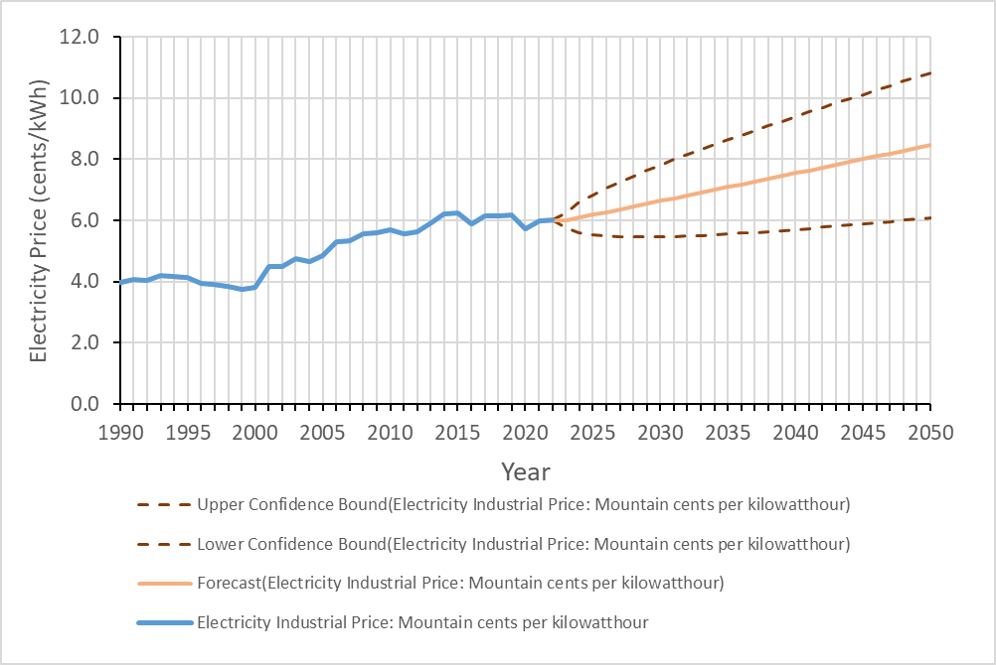
\includegraphics[width=.8\textwidth]{templates/images/Figure-EIA_Electricity_Forecast.png}
\caption[Electricity price forecast]{Price of electricity from the EIA Short-Term Energy Outlook \protect\citep{eia_short-term_2021}, forecast out to 2050.}
\label{fig:electricity_pricing}
\end{figure}

\subsection{Uncertainties}

The model described thus far takes a deterministic approach; parameter values are fixed to their most-likely values when performing the NPV calculation. A probabilistic approach replaces these static values with distributions and repeatedly samples from those distributions to capture an ensemble of results. This Monte Carlo-style simulation can provide a more realistic assessment of system performance.

However, all variables in the model have some underlying uncertainty, and defining distributions for every variable would add significant complexity to the model with diminishing returns. Variable selection can be performed using sensitivity testing to target the most impactful variables for uncertainty characterization. This helps balance model complexity with representativeness of the physical system. 

Recognizing the full probable range of possible variable values and the scenarios that trigger them requires a deep understanding of the scientific, engineering, and socio-technical elements influencing a system. For geothermal, subsurface characterization uncertainties play an important role, but so do uncertainties tied to public policy and market dynamics. The limited focus on the issues listed below should be considered fit-for-purpose for this thesis. Further analysis and discussion with subject matter experts on the local, state, and national levels is advised for similar analysis performed for an active geothermal project.

\subsubsection{Carbon Taxation}
\begin{wrapfigure}{R}{0.5\linewidth}
\centering
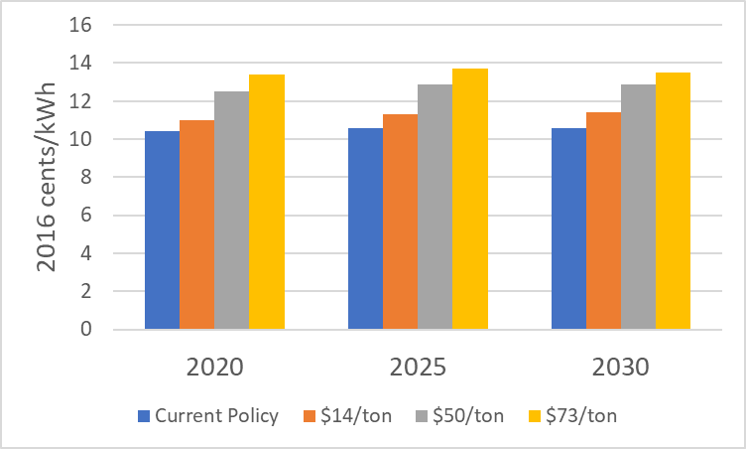
\includegraphics[scale=0.6]{templates/images/Figure-Carbon_Tax_Price_Impact.png}
\singlespacing
\caption[Carbon tax price impact]{National average retail electricity price changes with benchmark levels of carbon taxation, after \protect\citep[Fig.\ 30]{larson_energy_2018}.}
\label{fig:carbon_tax_pricing}
\end{wrapfigure}

One proposal for advancing the energy transition to more renewable and sustainable energy solutions involves a carbon tax levied on fossil fuels. The SIPA Center on Global Energy Policy at Columbia University recently studied three analytical scenarios based on federal agency benchmark taxation rates of \$14/ton, \$50/ton, and \$73/ton CO$_2$ equivalent with annual percentage rate increases of 3, 2, and 1.5\%, respectively \citep{larson_energy_2018} (Figure \ref{fig:carbon_tax_pricing}). Their analysis forecasts the impact on electricity pricing out to 2030, with relatively steady-state implications that depend on the specified carbon tax rate. In all taxation cases, electricity prices increase over the present-day, no-tax scenario, likewise boosting the value of a zero-emissions geothermal power relative to fossil fuel-based options. The selected value range for sensitivity testing was a 0-28\% increase in wholesale price, which matches Figure \ref{fig:carbon_tax_pricing}.

\subsubsection{Future Electrification}
NREL published a report earlier this year outlining the potential impact of heightened public trends away from non-electric sources of consumed energy, otherwise known as widespread electrification \citep{murphy_electrification_2021}. Some key findings include: (i) end-use natural gas consumption decreases, but so do natural gas prices, which can lead to an increase in natural gas-fueled power plants -- assuming no curtailments due to fossil fuel policies, (ii) deployment of renewables will intensify overall, and (iii) local resources, potentially including new renewable electricity generation facilities, will be relied on to mitigate the need for long-distance electricity transmission \citep{murphy_electrification_2021}.

\begin{wrapfigure}{R}{0.6\linewidth}
\centering
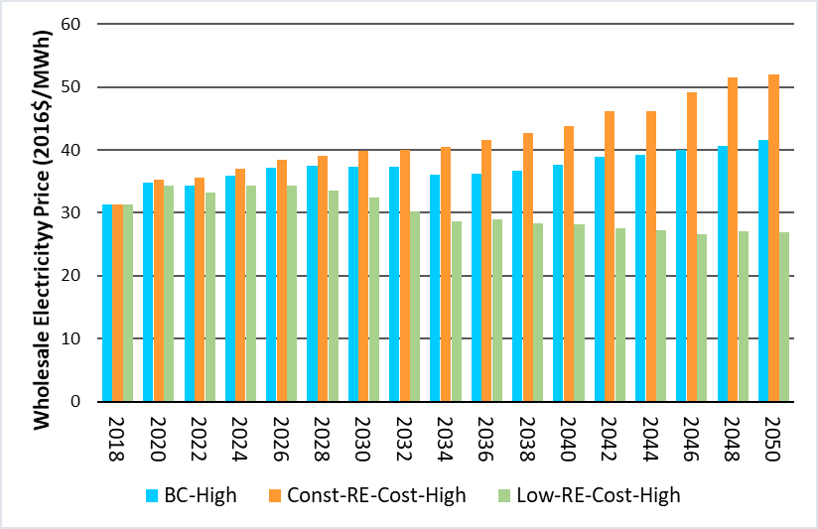
\includegraphics[scale=0.65]{templates/images/Figure-EFS_SIPA_Results.png}
\singlespacing
\caption[Electrification price impact]{Wholesale electricity price forecasts for high future electrification scenarios: base case (blue), constant renewable technology cost (orange), and low renewable technology cost (green). Cases are from the NREL Electrification Futures Study \protect\citep{murphy_electrification_2021}. Figure is adapted from interactive plots at https://cambium.nrel.gov/? project=fc00a185-f280-47d5-a610-2f892c296e51.}
\label{fig:EFS_electricification}
\end{wrapfigure}
The issue of national electrification is quite complex, particularly in the interplay between the natural gas market and renewables. Additional dependencies include infrastructure upgrades and development to handle growing capacity, as well as local effects (e.g., permitting, water or electrical transmission, community support) that act as enablers or hurdles to building a new renewable-fueled power plant or expanding on existing power facilities. One way to simplify a model representation of widespread electrification is to incorporate swings in electricity prices similar to the scenarios shown in Figure \ref{fig:EFS_electricification} with the caveat that other related factors (e.g., federal and state-level incentive programs or infrastructure improvements) can also influence the bottom line for a geothermal project. Based on NREL projections, wholesale electricity pricing in 2050 could vary from 0.65 to 1.25 times the prices recorded in 2018. Using the High Future Electrification (HFE) Base Case as a reference, prices are 25\% greater by 2050 for the HFE Constant Renewable Technology Costs case and prices drop by 35\% for the HFE Low Renewable Technology Costs case (Figure \ref{fig:EFS_electricification}). Therefore, +25\% and -35\% define the range of price factors used for sensitivity testing.

\subsubsection{Future Electrification}